%! TeX root = master.tex
% !TEX program = lualatex

\lecture{8}{14-04-2026}{Data Representations \& Processing}{}
\section{Data representation}
\subsection{Why ?}
\begin{enumerate}
\item Data heterogeneity: we cannot compare vectors of different dimensions (e.g, subtract $x_i \in \mathbb{R}^{200 \cdot 200 \cdot 3}$ and $x_j \in \mathbb{R}^{210 \cdot 223 \cdot 3}$, or compare speech samples of different length). 
\item Data size: A single, fairly small image is already a very long vector, so what about the size of a complete data set ?
\item Data noisiness: Not every piece of data encodes valuable information (E.g, for image recognition/text categorization: not all pixels/words are indicative of the class).
\item Some representations are better suited to certain tasks than others.
\end{enumerate}
The resulting representations can be directly used as input to an ML algorithm (applicable to all the methods we have seen so far, but in general to most machine learning algorithms).

\subsection{Attributes}
Attributes could be of different types: 
\begin{itemize}
  \item Categorical (e.g, sex: M, F, I)
  \item Real (continuous) (e.g, length in mm)
  \item Integer (discrete)
\end{itemize}

\subsection{Bag of Words}
To represent text document we will use bag of words, it consists of a mapping of each words to the number of it's occurence in the text.

\subsubsection{Constructing a dictionary}
\begin{enumerate}
  \item Consider only the words that appear in the dataset (n samples)  
  \item Do not consider the too common words, e.g., “the”, “a”, “to”,
“it”, “is”, “for”,…
\end{enumerate}

\subsubsection{Vector representation of BoW}
With $D$ words in the dictionary, each sample can be representd as a vector in $\mathbb{R}^D$.

\subsubsection{Histograms}
The final BoW representation is a histogram such that \[
  x_1^{(d)} \in [\ 0,1]\
\]
\[
  \sum_{d=1}^{D} x_1^{(d)} = 1
\]

\paragraph{Example}
2 samples :

(1) John likes to watch movies. Mary likes movies too. 

(2) John also likes to watch football games. 

Corresponding counts : 

BoW1 = \{ \textcolor{red}{"John"}:1, \textcolor{red}{"likes"}:2, \textcolor{red}{"to"}:1, \textcolor{red}{"watch"}:1, \textcolor{red}{"movies"}:2, \textcolor{red}{"Mary"}:1, \textcolor{red}{"too"}:1\};

BoW2 = \{\textcolor{red}{"John"}:1, \textcolor{red}{"also"}:1, \textcolor{red}{"likes"}:1, \textcolor{red}{"to"}:1, \textcolor{red}{"watch"}:1, \textcolor{red}{"football"}:1, \textcolor{red}{"games"}:1\};
 
Our dictionary is all the words appearing in the 2 samples after removing "to" : 
  
\quad \quad \quad \quad \text{\textcolor{red}{"John", "likes", "watch", "movies", "Mary", "too", "also", "football", "games"}}

The vector representation of the BoWs are ($D = 9$) : \[
  \tilde{x}_1 = \begin{pmatrix}
    1 & 2 & 1 & 2 & 1 & 1 & 0 & 0 & 0   
  \end{pmatrix}
\]
\[
  \tilde{x}_2 = \begin{pmatrix}
    1 & 1 & 1 & 0 & 0 & 0 & 1 & 1 & 1
  \end{pmatrix}
\]
And the histogram are \[
  x_1 = \begin{pmatrix}
    1/8 & 1/4 & 1/8 & 1/4 & 1/8 & 1/8 & 0 & 0 & 0 
  \end{pmatrix}
\]
\[
  x_2 = \begin{pmatrix}
    1/6 & 1/6 & 1/6 & 0 & 0 & 0 & 1/6 & 1/6 & 1/6
  \end{pmatrix}
\]

\subsection{Bag of visual words}
For images we could adapt the BoW, as objects are made of common parts/patches (can be thought of as visual words), we could use them instead of words.
\subsection{Visual dictionary}
\begin{enumerate}
  \item Extract patches from all images
  \item Group the patches based on similarity to optain prototypes that act as dictionary words (The center of each cluster (group) is taken as a visual word)
  \item For each patch in an image
    \begin{itemize}
      \item find the nearest visual word
      \item add one to the corresponding element in a BoW vector
    \end{itemize}
  \item Normalize the BoW vectors to obtain histograms
\end{enumerate}


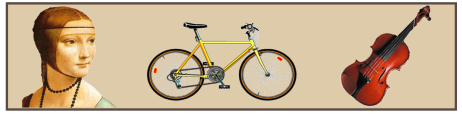
\includegraphics[width=0.3\linewidth]{images/img_20260414_002236.png} \to 
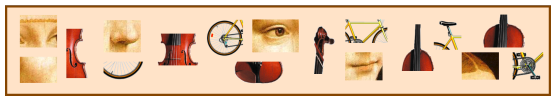
\includegraphics[width=0.35\linewidth]{images/img_20260414_002252.png} \to 
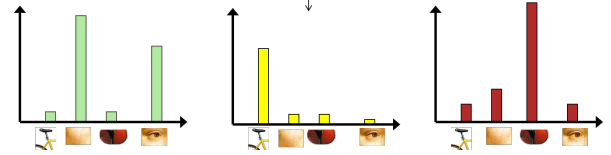
\includegraphics[width=0.33\linewidth]{images/img_20260414_002259.png}

\subsection{Data pre-processing}
Even with a good representation, the data might benefit from
being pre-processed. (e.g,  Some attribute values are missing/noisy or the feature dimensions are of incommensurate magnitudes)

\subsubsection{Missing data}
Attributes values that are not recorded (E.g., the Air Quality UCI dataset contains missing values, which are tagged
with a -200 value)

Potential solutions:

\begin{itemize}
  \item Ignore the corresponding sample
  \item Fill in the missing values with a global constant
  \item Fill in the missing values with the corresponding attribute average over the
dataset
  \item Fill in the missing values with the corresponding attribute average over the
samples belonging to the same class
\end{itemize}

\subsubsection{Noisy data}
Noise: Random measurement error

Incorrect values : Faulty data collection, Data entry problems, Data transmission problems

Other problems : Duplicate entries, Inconsistent data

\subsubsection{Cleaning noisy data}
\begin{enumerate}
  \item Cleaning by \textbf{binning}:

For each attribute:
\begin{enumerate}
  \item Sort the data 
  \item Partition it into bins 
\item Smooth the data by taking the bin means or medians
\end{enumerate}

E.g:
\begin{itemize}
  \item \textbf{Data :} 0, 4, 12, 16, 16, 16, 18, 24, 26, 28 
  \item \textbf{Equal width}
  \begin{itemize}
    \item[] \begin{tabular}{l@{\hspace{2cm}}l}
      Bin 1: 0, 4          & $[-\infty, 10)$ \\
      Bin 2: 12, 16, 16, 18 & $[10, 20)$ \\
      Bin 3: 24, 26, 28    & $[20, +\infty)$ \\
    \end{tabular}
  \end{itemize}
  \item \textbf{Equal frequency}
  \begin{itemize}
    \item[] \begin{tabular}{l@{\hspace{2cm}}l}
      Bin 1: 0, 4, 12      & $[-\infty, 10)$ \\
      Bin 2: 16, 16, 18    & $[14, 21]$ \\
      Bin 3: 24, 26, 28    & $[21, +\infty)$ \\
    \end{tabular}
  \end{itemize}
\end{itemize}
\item Clustering : Detect outliers as the clusters with too few elements and remove these
samples

\item Leverage human knowledge: remove values that have non-sense (e.g, Blood pressure cannot be 0, salary cannot be negative).
\end{enumerate}

\subsection{Data normalization}
Goal: Scale each individual attribute/feature dimension to fall
within a specified range. 

\subsubsection{Min-max normalization}
For each feature dimension $d$, compute the normalized feature
\[
  \tilde{x}_i^{(d)} = \frac{x_i^{(d)} - x_{min}^{(d)}}{x_{max}^{(d)} - x_{min}^{(d)}}
\]
where $x_{min}^{(d)} = \min_{i=1}^N x_i^{(d)}$ and $x_{max}^{(d)} = \max_{i=1}^N x_i^{(d)}$

\subsubsection{z-score normalization}
For each feature dimension $d$, compute the normalized feature
\[
  \tilde{x}_i^{(d)} = \frac{x_i^{(d)} - \mu^{(d)}}{\sigma^{(d)}}
\]

where $\mu^{(d)} = \frac{1}{N} \sum_{i=1}^{N} x_i^{(d)}$

$\sigma^{(d)} = \sqrt{\frac{1}{N}\sum_{i=1}^{N} (x_i^{(d)} - \mu^{(d)})^2}$

\subsubsection{max normalization}
For each feature dimension $d$, compute the normalized feature \[
  \tilde{x_i}^{(d)} = \frac{x_i^{(d)}}{x_{max}^{(d)}}
\]
where $x_{max}^{(d)} = \max_{i=1}^N \left|x_i^{(d)}\right|$

\subsubsection{decimal scaling normalization}
For each feature dimension $d$, compute the normalized feature \[
\[
  \tilde{x_i}^{(d)} = \frac{x_i^{(d)}}{10^k}
\]
where $k$ is the smallest integer such that $\max_{i=1}^N \left| \tilde{x}_i^{(d)}\right| \leq 1$

\subsubsection{Remark}

For all data processing techniques, the normalized (or cleaned) features are then used as input to an ML algorithm
\begin{itemize}
  \item  Normalization is not aways necessary, and may or may not help depending
on the data at hand and on the chosen ML algorithm
\end{itemize}

Data representations and data cleaning/normalization acts on the individual samples
\begin{itemize}
  \item Although the normalization statistics come from the whole training set
\end{itemize}

Nevertheless, even with good representations, the data set
itself might make from learning more difficult (imbalanced data).

\subsection{Imbalanced data}
If a class is very majoritary, the classifier learn to predict always this class (high accuracy but predict poorly on the minoritary class) instead of learning patterns. 

Two type of imbalance : 
\begin{itemize}
  \item Between-class imbalance : one class dominates 
  \item Within-class imbalance : bad spatial repartition of the samples inside a class
\end{itemize}

\begin{center}
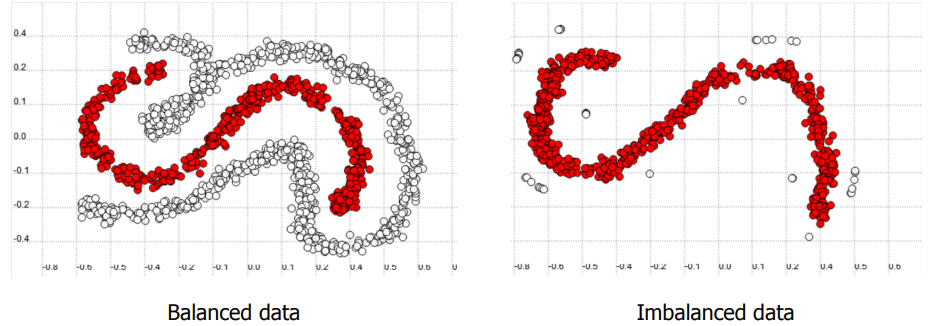
\includegraphics[width=0.5\linewidth]{images/img_20260414_011401.png}
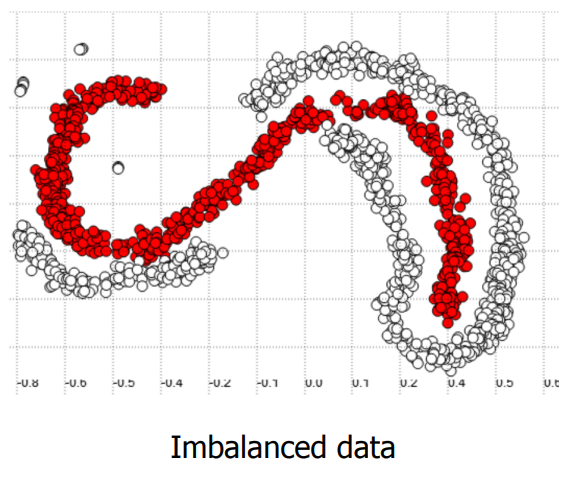
\includegraphics[width=0.2125\linewidth]{images/img_20260430_182033.png}
\end{center}

\subsubsection{Learning with imbalanced data}
Two main approaches: 
\begin{itemize}
  \item One that act on the data: Sampling Methods 
  \item One that act on the cost function: Cost-Sensitive Methods
\end{itemize}

\subsubsection{Sampling Methods}
Two ways to compensate the lack of data:
\begin{itemize}
  \item Increase the Dataset, by generating new datapoints for the smallest class   
  \item Decrease the Dataset, by removing redundant datapoints from the largest class
\end{itemize}

\subsubsection{Decrease the data: Undersampling}
Naive (random) undersampling:
\begin{itemize}
  \item Randomly remove samples from the largest class until you obtain a
balanced data set 
\item Drawback: May remove important samples
\end{itemize}

More clever undersampling:
\begin{itemize}
  \item Remove the redundant samples 
  \item Good if the class to undersample is densely populated (e.g., lowdimensional representation because of the curse of dimensionality)
\begin{center}  
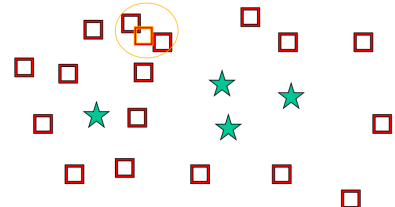
\includegraphics[width=0.4\linewidth]{images/img_20260414_012315.png}
\end{center}

\end{itemize}
\subsubsection{Increase the data: Oversampling}
Naive (random) oversampling: \begin{itemize}
  \item Replicate the data samples from the smallest class until you obtain a
balanced data set 
\item Drawback: May lead to overfitting
\end{itemize}

More clever oversampling:  \begin{itemize}
  \item Create new data samples based on neighboring existing ones 
  \item This may create noisy samples

\begin{center} 
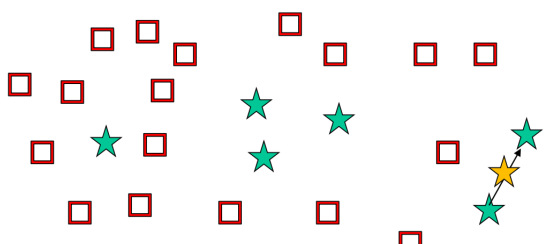
\includegraphics[width=0.45\linewidth]{images/img_20260414_012533.png}
\end{center}

\end{itemize}

\subsubsection{Empirical risk}
Given $N$ training samples $\left\{(x_i, y_i)\right\}$, the empirical risk is defined as \[
  R(\left\{x_i\right\}, \left\{y_i\right\}, w) = \frac{1}{N}\sum_{i=1}^{N} l(\hat{y}_i, y_i)
\]
where $\left\{x_i\right\}$ and $\left\{y_i\right\}$ are the sets of training inputs and labels, respectively. 

In general, each loss term $l(\hat{y_i}, y_i)$ has the same influence, with imbalanced data, this means that most of the empirical
risk comes from the largest class.

\subsubsection{Sample re-weighting}

A simple solution to this problem consist of re-weighting the
samples, to put more emphasis on the rare class. 

This gives an empirical risk of the form \[
  R(\left\{x_i\right\}, \left\{y_i\right\}, w) = \frac{1}{N}\sum_{i=1}^{N} \beta_i l(\hat{y}_i, y_i)
\]
where $\beta_i$ is the weight for sample $i. 

This strategy is quite general (e.g, it applies to least-square classification, logistic regression, SVM (in the three cases, since the weights are fixed during
optimization, the respective optimization problems remain convex and can thus be solved to optimality)).

\subsubsection{From handcrafted representations to learned ones}
As the representations and data processing strategies we have
discussed so far were all manually designed, it doesn't guarantee that they are the best
representations for the task at hand. 

Ideally, one would therefore like to learn the representation
jointly with the classifier \to neural networks.
